%%%%%%%%%%%%%%%%%%%%%%%%%%%%%%%%%%%%%%%%%%%%%%%%%%%%%%%%%%%%%%%%%%%%%%%%%%%%%%%%
%nscience.tex: Chapter on theory:
%%%%%%%%%%%%%%%%%%%%%%%%%%%%%%%%%%%%%%%%%%%%%%%%%%%%%%%%%%%%%%%%%%%%%%%%%%%%%%%%
\chapter{Physics of the Standard Model and Left-Right Symmetric Extensions}
\label{ch:theory}

\section{Development of the Standard Model}

The standard model of particle physics, or simply the standard model, encapsulates discoveries in physics stretching well over a century and was chiefly formulated by Weinberg, Glashow, and Salam \cite{PhysRevLett.19.1264}\cite{nla.cat-vn956113}.  The standard model combines electromagnetism, the nuclear weak force, and the nuclear strong force to describe the properties and interactions of all matter, excluding gravity.

At the beginning of the 20th century, Einstein and Lorentz developed special relativity, Maxwell's early work developing the four equations of electricity and magnetism was shown to be fundamentally Lorentz invariant, like the speed of light. \cite{1898KNAB1427L}\cite{doi:10.1002/andp.19053221004}.  In the 1920s Dirac created the first quantum field-theory, recreating Maxwell's equations for relativistic and quantum cases \cite{doi:10.1098/rspa.1928.0023}.  With this reformulation, the first new particles, anti-particles, were predicted and the observed fundamental spin of particles was explained.  These predictions of Dirac were confirmed by Anderson 1932 with Cosmic-rays seen decaying to oppositely charged electrons (anti-electrons, or positrons) \cite{PhysRev.43.491}.  Feynman developed Quantum Electrodynamics (QED) and with the work of others created a completely consistent theory of all electromagnetic interactions in the 1940s \cite{PhysRev.76.769}.

The weak nuclear force was first motivated studying beta decay.  Pauli noticed a lack of conservation of momentum in the decay, necessitating an extremely light and unseen particle, which was called "little neutral one", or neutrino.  This allowed for momentum conservation and Fermi proposed a contact interaction between a proton, electron, and the neutrino.  This interaction between four-fermions successfully predicted the spectrum of beta decay \cite{Fermi1934}, though it has since been updated to include the weak boson, only directly observable at much higher energies than nuclear decays.

Further study of the weak force into the 1950s lead to a puzzle regarding the conservation of parity.  Two particles were discovered, \ensuremath{\tau} and \ensuremath{\theta} which were observed identical except for their parity \cite{osti_4356004}.  Lee and Yang instead proposed that these were the same particles, which instead violated parity symmetry in its decay \cite{PhysRev.104.254}.  The beta decay of \cobaltsixty by Wu confirmed the parity violating nature of the weak force \cite{articlePARITYTEST}.  Meson decays in a storage ring were also studied, revealing more evidence for parity violation \cite{articlePARITYFAIL}.  Sudarshan, Marshak, Feynman, and Gell-Man all worked to develop a new model for the weak force which would include parity-violation.  This was the \vminusa  model, vector minus axial vector, as axial vectors, like chirality, do not transform the same under parity as regular vectors \cite{1898KNAB1427L}\cite{PhysRev.109.193}.

Parallel to the work developing the \vminusa formulation, Yang and Mills created a non-Abelian gauge theory describing the weak force in 1954.  This replaced the contact interaction, first theorized by Fermi, with a charge 1, spin 1 particle as an intermediary \cite{PhysRev.96.191}.  This theory was physically impossible for the weak force, as the weak boson proposed was massless, requiring the weak force to be of infinite range, like electromagnetism.  Glashow modified the proposed theory in 1960.  He added the \vminusa model of Sudarshan and Marshak and combined Feynman's QED, describing it all in a single theory with the gauge group \SUtwoUone \cite{GLASHOW1961579} and predicting an additional heavy boson mixing the photon.  The weak \SUtwoL group only couples two left-handed chiral states.  The last piece of the puzzle was completed by Weinberg and Salam \cite{PhysRevLett.19.1264}\cite{nla.cat-vn956113}.  They added the Brout, Englert, and Higgs mechanism \cite{PhysRevLett.13.321}\cite{PhysRevLett.13.508} which gives mass to vector bosons in the Yang-Mills theory, and predicted an additional boson, the Higgs, not to be discovered until 2012 \cite{higgs2012ATLAS}\cite{higgs2012CMS}.

Parallel to the work in what is called the electro-weak sector of the standard model, cosmic rays and nuclear interactions were providing evidence for another fundamental force of a different sort, the strong nuclear force.  Starting in 1947 cosmic ray events studied in cloud chambers lead to the discovery of particles such as kaons \cite{1947Natur.160..855R}.  These particles were strange, as they seemed to an additional quantum number no other particles did.  Not until the 1960s did Gell-Mann and Zweig propose a symmetry group \SUthree to explain this \cite{osti_4082875} \cite{Zweig:352337}.  This quark model theorized that all strongly interacting particles were composed of fundamental quarks, three observed and one theorized.  The extra property kaons and other mesons like it, was that they were made partly of "strange quarks".  More typical mesons, as well as protons and neutrons, were made of "up" and "down" quarks.  The theory predicted one more quark, which was discovered and named "charm", though it was later extended to include two more, the "bottom" and "top" quarks.  The interactions in the quark model are based on color charge and only color neutral particles can be freely propagating.  Adding the \SUthree group to the electro-weak sector gives the complete standard model picture, a \SUthreeSUtwoUone symmetry group.

Every particle predicted in the standard model has now been observed.  The first indirect observation of the \Z was in 1973 at CERN \cite{HASERT1973121}.  The charm quark, confirming quark theory, was discovered at BNL and SLAC and then the bottom quark was soon discovered by the E288 experiment \cite{Aubert:1974js}\cite{Augustin:1974xw}\cite{Herb:1977ek}.  In 1983 the weak bosons were directly discovered by the UA1 and UA2 experiments at CERN \cite{Arnison:1983mk}\cite{Bagnaia:1983zx}\cite{Arnison:1983rp}\cite{Banner:1983jy}.  The top quark, the heaviest particle in the standard model, was discovered in 1995 at FNAL by the D0 and CDF groups using the Tevatron \cite{d4eca9bf1d5f49f3a4adc794f80c0a00}\cite{Abachi:1994td}.  Finally, the Higgs boson was first discovered by \CMS and ATLAS at CERN in 2012 with the \LHC.  In addition to the successful discover of all the particles in the standard model, the model allows for extremely precise verification of physical constants.  An example being the gyromagnetic ratio of the muon, which has been calculated to within one part in one ten-billionth, and agrees with measurements to better than one part in one billion \cite{PhysRevD.98.030001}.

\section{Components of the Standard Model}
The Standard Model of particle physics combines three of the four discovered fundamental forces in the universe: the electromagnetic force, the weak force, and the strong force.  There has yet to be a successful quantum field theoretic composition of gravity, so it is not yet included.

The Standard Model describes the fundamental particles and forces in nature.  Each fundamental force has particles which interact with, and the particles which carry the force in exchange between interacting particles.  Each interaction in the standard model can be described using Lie algebra, allowing the model to be described as combinations of groups.  Each fundamental force is also constructed around a fundamental preservation of certain quanta.

\begin{figure}[!htbp]
    \centering
    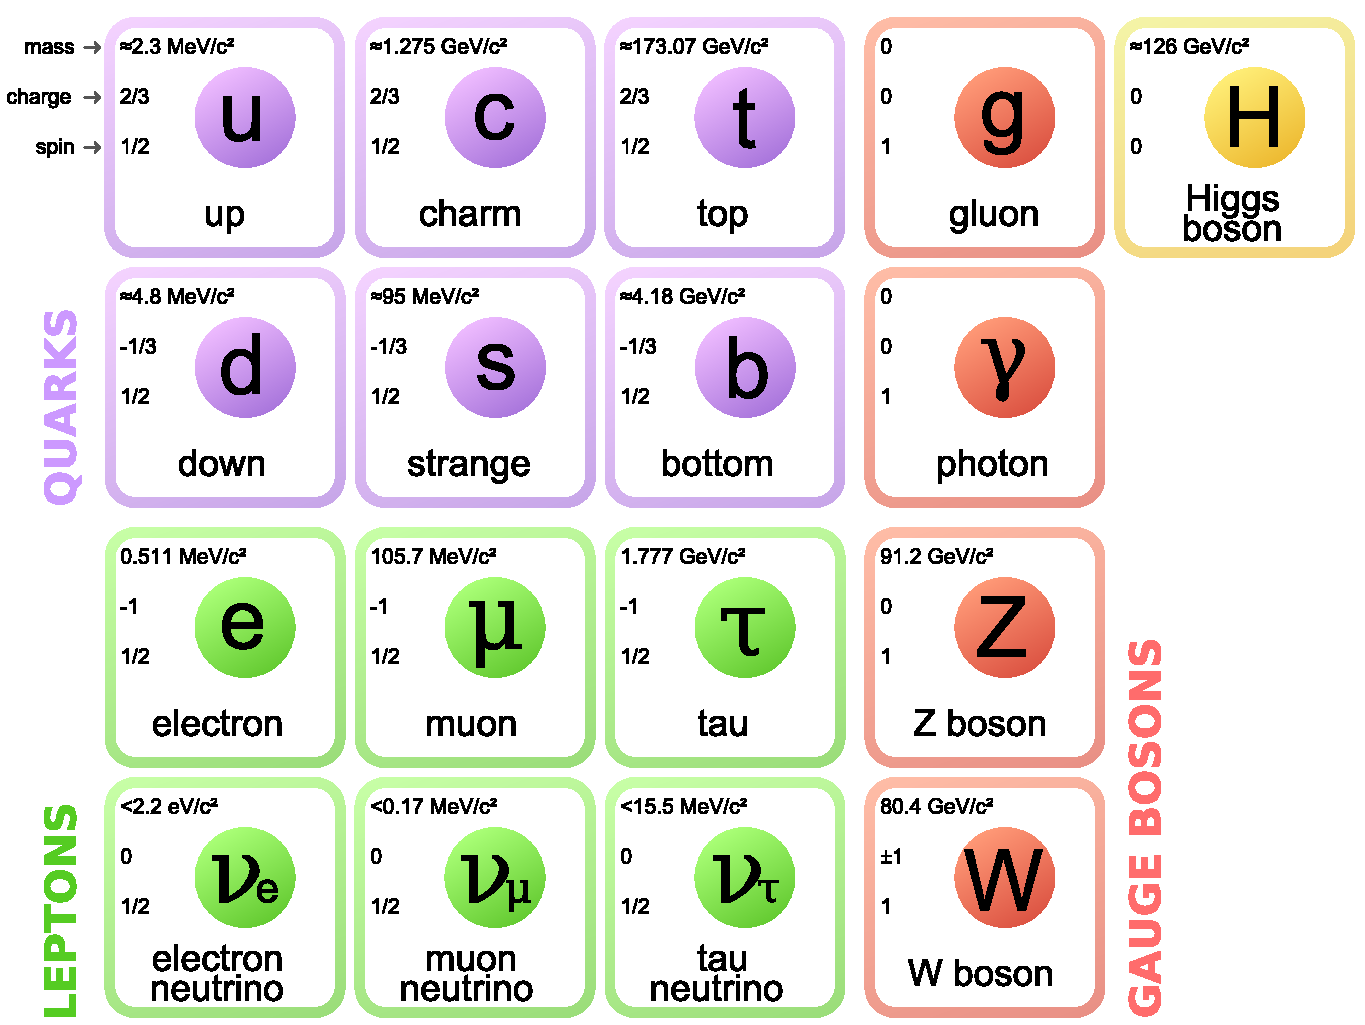
\includegraphics[width=\textwidth]{figures/standard_model.pdf}
    \caption[Diagram of the particles in the standard model.]
       {The particles of the Standard Model.  The quarks are shown in purple, the leptons in green, the exchange particles in red, and the Higgs is shown in yellow.  Each particle's name, mass, charge, and spin is also shown.}
    \label{fig:ParticleTable}
\end{figure}

A diagram of the standard model and each particle's properties are shown in \ref{fig:ParticleTable}.  There are three kinds of particles in the standard model: quarks, leptons, and gauge bosons.  Quarks and leptons make up all of matter, and are fermions, while the gauge bosons define the fundamental force interactions and are bosons. There are three generations of quarks and leptons, each heavier than the last.  The lightest generation being the up and down quarks and the electron (and electron neutrino).  These particles make up all stable matter in the universe.  Heavier generations have the same properties as these, though they all can decay via the weak force into lighter generations. 
The quarks interact with all of the forces described in the standard model.  They have \ensuremath{\mp\frac{1}{3}} or \ensuremath{\pm\frac{2}{3}} electric charge and a spin of \ensuremath{\frac{1}{2}}.
The leptons are the electron, muon, and tau, along with each's neutrino.  Each lepton has a charge of \ensuremath{-1} and a spin of \ensuremath{\frac{1}{2}}.  The neutrinos are not charged however, and are of unknown mass.  The nature of neutrino mass is not in the standard model, and will be discussed further in section \ref{sec:LRStheory}.
The five bosons of the standard model emerge from the quantum field theories that define it.  The gluon solely interacts with quarks and gluons and is part of the \SUthree group.  The photon (massless) and Z bosons (massive) are part of a superposition of weak-flavor neutral fermion anti-fermion interactions in the electro-weak sector, and the W boson comes from the axial vector, symmetry breaking part of the electro-weak sector.  Its interactions with matter involve weak-flavor transitions, most commonly seen on earth as \ensuremath{\beta} decay. The Higgs Boson, comes from the Higgs field, giving the weak bosons, W and Z mass, and additionally provides a mechanism for fermion mass.  These interactions will be discussed further in the following subsections.

\subsection{The Strong Force}
The strong nuclear force, called Quantum Chromodynamics (QCD), contained in the standard model describes a complicated 3 flavor interaction \SUthree. Each flavor is described as a "color" or "color charge": red, green, and blue. Each quark may have one of these colors, anti-quarks have anti-colors. The intermediating particle, the gluon, carries pairs of color anti-colors. QCD requires the conservation of this color in all interactions. In addition to conservation color, free particles must be color neutral (white). This feature, called confinement, arises from the fact that as quarks are separated from each other, additional quarks can form from the potential energy in the strong field. This prevents any bare quarks or gluons being visible. Any quark or gluon with sufficient energy to travel away from an interaction will form more colored particles in between it's past partner. This spray of hadrons is called a "jet". Color neutral quark combinations are generally mesons, which are color, anti-color quark pairs, or baryons which are three quark, red-green-blue combinations, all are called hadrons.

\subsection{The Electro-weak Interaction}
The electro-weak interaction comes from the combination of two groups \SUtwoUone . This gives four vector bosons.  Three are from the \SUtwoL group: \ensuremath{A^i} with \ensuremath{i\in\{1,2,3\}}.  Tne last is from the \Uone group: \ensuremath{B}. The physical states observed, the W, Z and \ensuremath{\gamma} are linear combinations of \ensuremath{A^i} and \ensuremath{B}. These combinations define the W boson as

\begin{equation}\label{eq:Wboson}
    W_{\mu}^{\pm}
    \equiv  
    \frac{1}{\sqrt{2}}
    \left(
    A_{\mu}^{1}
    \pm
    iA_{\mu}^{2}
    \right)
\end{equation}

The Z and photon combinations are:

\begin{equation}\label{eq:Z}
    Z_{\mu}
    \equiv  
    \sin{\theta_W}
    B_{\mu}
    -
    \cos{\theta_W}
    A_\mu^3
    \end{equation}
\begin{equation}\label{eq:photon}
     A_{\mu}
    \equiv  
    \cos{\theta_W}
    B_{\mu}
    -
    \sin{\theta_W}
    A_\mu^3
\end{equation}

The \vminusa composition of the standard model weak force is parity violating, and removes the possibility of right-handed weak interactions.  Thus, all neutrinos and all interactions with the W boson are only with left-handed particles. From the moment this theory was developed, physicists have worked at ways to restore parity symmetry with a right-handed weak interaction \cite{lr}\cite{lr1}.

\subsection{The Brout-Englert-Higgs Mechanism}
 
\section{Left-Right Symmetric Extensions to the Standard Model}
\label{sec:LRStheory}
The left-handed nature of the weak force \SUtwoL, and the left-right symmetry of every other group, leads to a desire to complete the symmetry of the standard model by adding a right-handed component to the weak force.  Completing the standard model has additional functional benefits stemming allowing for neutrinos to have mass.  By the see-saw method, the currently observed left-handed neutrinos can be very light, countered by very heavy right-handed neutrinos.  Naturally, the symmetry would have to be broken at some energy level, allowing for the currently observed asymmetry at low energies.

Left-right symmetric extensions (LRS) models would require adding an additional symmetry group to the standard model or simply making the standard model a part of a larger symmetry like \SUfive or \Oten.  To simplify discussing the theory, we'll focus on the simplest extension.  Here, the electro-weak sector simply gains another \SUtwo group, make it \SUlrs.

Adding this extension creates three additional particles, the \WR and \NR, which this thesis is about the search for, and a partner to the \ensuremath{Z}, the \Zprime.  We can also assume that left and right-handed interactions have the same coupling strength.  While this also is not required in a more complicated LRS model, it is reasonable to assume it for the search.

The right-handed extension additionally complicates the Higgs sector, requiring at least a Higgs doublet to couple to the right and left handed weak bosons independently.



\subsection{Right-Handed Neutrino Jets}
While LRS models do not give any suggestions for the \NR - \WR mass relationship, searches where the \NR is lighter, but of the same order of magnitude as the \WR have been performed cite T13-19.  It is however, just as possible that the mass of the \NR be significantly lighter than the \WR mass \ensuremath{m_{\NR} / m_{\WR} \leq 0.1}.  In this situation the neutrinos will be produced with large transverse momentum, and the lepton and two quarks from the \NR decay will be collimated in the lab frame.  A detailed discussion of \NR "jets" can be found in \cite{nrjets}.
\subsection{Experimental Study of LRS Models}

While right-handed extensions to the weak force have been studied and searched for for a long time, no experimental evidence has given evidence for them.  In addition, the models themselves have too many free parameters to make any exact prediction.

\subsection{New Particle Production at the LHC}
As the highest energy particle collider created to date, the LHC has the possibility to reach collision energy levels where new, previously unobserved particles could be created.  The \LHC and \CMS will be described further in the \label{experiment_chapter}.

In a high energy particle collision, the energy of the collision available to produce new particle mass is defined as:
\begin{equation}\label{eq:roots}
    \sqrt[]{s}
    =   
    \sqrt[]{
       \left( \sum_{i=1}^{2} E_i \right) ^ 2
       -
       \left( \sum_{i=1}^{2} \boldmath{p}_i \right) ^ 2
    }
\end{equation}
Where the square sum of each particle's energy is subtracted from the square sum of each particle's momentum.

While the LHC operates at a \rootsthirteen , this is the nominal collision energy between two protons, which are hadrons.  Each collision actually consists of interactions between quarks and exchanged gluons within the proton.  These contents of the proton are called partons.  The probability of a specific parton-parton interaction with a certain fraction of the proton momentum varies.  The probability of a parton-parton collision with near \rootsthirteen is exceeding small.  While the parton interactions contain only a fraction of the total collision momentum, there signatures could still stand above background.
 
%%%%%%%%%%%%%%%%%%%%%%%%%%%%%%%%%%%%%%%%%%%%%%%%%%%%%%%%%%%%%%%%%%%%%%%%%%%%%%%%

%%%%%%%%%%%%%%%%%%%%%%%%%%%%%%%%%%%%%%%%%%%%%%%%%%%%%%%%%%%%%%%%%%%%%%%%%%%%%%%%
